\begin{problem}{1.1}{problem1_1}

A simplified $m$ longitudinal motion of an underwater vehicle can be described by
\begin{equation}
	m \ddot{x} + k \dot{x} |\dot{x}| = u
\end{equation}
where $x$ is the position of the vehicle, $u$ is the control input (a force that is provided by a propeller), $m$ is the mass of the vehicle, and $k > 0$ is the drag coefficient. Assuming the value of $m$ is known exactly, the drag coefficient is bounded $k_1 \leq k \leq k_2$, and the position and its derivative (velocity) $x, \dot{x}$ are measured:

\begin{enumerate}[label=\textbf{\alph*)}]
	\item Obtain a state system model of the vehicle using $x_1 = x, \, x_2 = \dot{x}$ as the state variables.
	\item Design a conventional sliding mode control law $u$ that drives $x_1, x_2 \rightarrow 0$ as time increases.
	\item Simulate the control system for $x_1(0) = 2\,\text{m}$, $x_2(0) = 0.5\,\text{m/s}$, $m = 4\,\text{kg}$, and $k = 1.5 + 0.4 \sin(2t)\,[\text{kg/ms}]$. Plot the time histories of the sliding variable, the control function $u$, the position $x_1$, and the velocity $x_2$.
	\item Identify the quantities that reach zero in finite time and the ones that approach zero asymptotically.
\end{enumerate}

\textbf{Hint:} The function $k\dot{x}|\dot{x}|$ can be bounded as
\[
	|k\dot{x}|\dot{x}|| \leq k_2 \dot{x}^2 = 1.9 \dot{x}^2.
\]

\end{problem}

\begin{solution}{}{solution1_1}
	\begin{enumerate}[label=\textbf{\alph*)}]
		\item Using the state variables \( x_1 = x \) and \( x_2 = \dot{x} \), the dynamic model of the vehicle can be expressed as:

		      \begin{equation*}
			      \begin{aligned}
				      \dot{x}_1 & = x_2,                                         \\
				      \dot{x}_2 & = \frac{1}{m} \left( -k x_2 |x_2| + u \right).
			      \end{aligned}
		      \end{equation*}

		\item Define the sliding surface as:
		      \[
			      \sigma = x_2 + c x_1, \quad c > 0,
		      \]
		      with its time derivative given by:
		      \[
			      \dot{\sigma} = c \dot{x}_1 + \dot{x}_2 = c x_2 + \frac{1}{m} \left( -k x_2 |x_2| + u \right).
		      \]

		      Consider the following Lyapunov candidate function:
		      \[
			      V = \frac{1}{2} \sigma^2,
		      \]
		      which has the time derivative:
		      \[
			      \dot{V} = \sigma \dot{\sigma} = \sigma \left( c x_2 + \frac{1}{m} \left( -k x_2 |x_2| + u \right) \right).
		      \]

		      Choose the control input as:
		      \[
			      u = m(-c x_2 + v),
		      \]
		      so that:
		      \[
			      \dot{V} = \sigma \left( -\frac{k}{m} x_2 |x_2| + v \right).
		      \]

		      Using the provided bound on the nonlinear term from the hint:
		      \[
			      |k x_2 |x_2|| \leq k_2 x_2^2 = 1.9 x_2^2,
		      \]
		      we can bound the derivative of \( V \) as:
		      \[
			      \dot{V} \leq |\sigma| \frac{1.9}{m} x_2^2 + \sigma v.
		      \]

		      To dominate the first term and ensure convergence, choose:
		      \[
			      v = -\left( \rho + \frac{1.9}{m} x_2^2 \right) \text{sign}(\sigma),
		      \]
		      where \( \rho > 0 \) is a design parameter.

		\item The simulation of the control system using $c=2$ and $\rho =2$ yields the following results:
		      \begin{figure}[H]
			      \centering
			      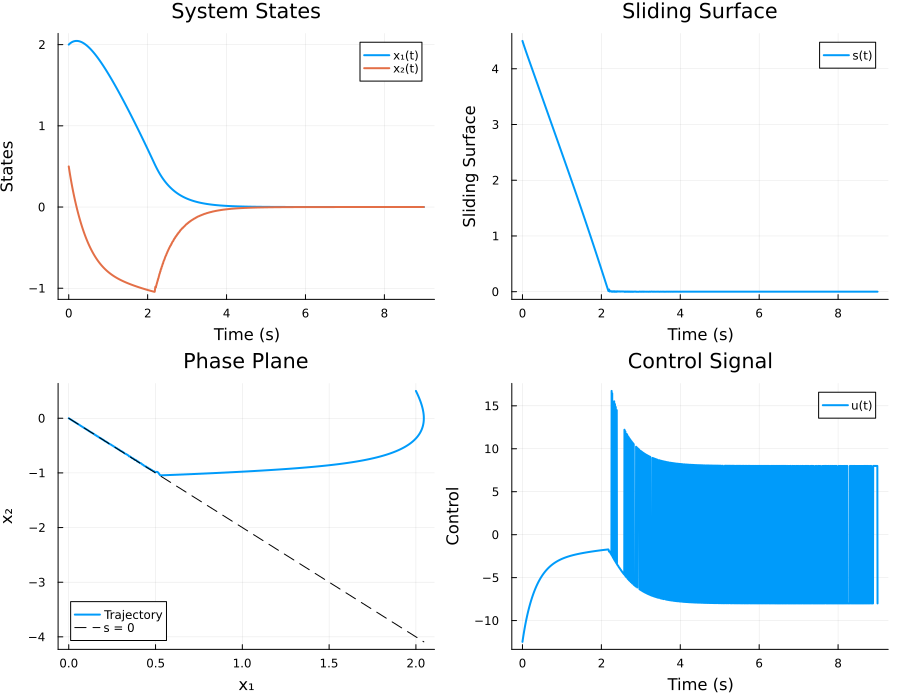
\includegraphics[width=1\textwidth]{img/problem1_1.png}
			      \caption{Simulation results for the sliding mode control system.}
			      \label{fig:problem1_1}
		      \end{figure}
        \item We can observe that the sliding variable \( \sigma \) reaches zero in finite time, indicating that the system enters the sliding mode, while the states \( x_1 \) and \( x_2 \) approach zero asymptotically. 

	\end{enumerate}
	\qed
\end{solution}